\documentclass[a4paper]{article}

\setlength{\parskip}{0.1em}
\usepackage{ifthen}
\usepackage{amssymb}
\usepackage{multicol}
\usepackage{graphicx}
\usepackage[absolute]{textpos}

\usepackage[noload]{qtree}
%\usepackage{xspace,rotating,calligra,dsfont,ifthen}
\usepackage{xspace,rotating,dsfont,ifthen}
\usepackage[spanish,activeacute]{babel}
\usepackage[utf8]{inputenc}
\usepackage{pgfpages}
\usepackage{pgf,pgfarrows,pgfnodes,pgfautomata,pgfheaps,xspace,dsfont}
\usepackage{listings}
\usepackage{multicol}


\makeatletter

\@ifclassloaded{beamer}{%
  \newcommand{\tocarEspacios}{%
    \addtolength{\leftskip}{4em}%
    \addtolength{\parindent}{-3em}%
  }%
}
{%
  \usepackage[top=1cm,bottom=2cm,left=1cm,right=1cm]{geometry}%
  \usepackage{color}%
  \newcommand{\tocarEspacios}{%
    \addtolength{\leftskip}{5em}%
    \addtolength{\parindent}{-3em}%
  }%
}

\newcommand{\encabezadoDeProc}[4]{%
  % Ponemos la palabrita problema en tt
%  \noindent%
  {\normalfont\bfseries\ttfamily proc}%
  % Ponemos el nombre del problema
  \ %
  {\normalfont\ttfamily #2}%
  \ 
  % Ponemos los parametros
  (#3)%
  \ifthenelse{\equal{#4}{}}{}{%
  \ =\ %
  % Ponemos el nombre del resultado
  {\normalfont\ttfamily #1}%
  % Por ultimo, va el tipo del resultado
  \ : #4}
}

\newcommand{\encabezadoDeTipo}[2]{%
  % Ponemos la palabrita tipo en tt
  {\normalfont\bfseries\ttfamily tipo}%
  % Ponemos el nombre del tipo
  \ %
  {\normalfont\ttfamily #2}%
  \ifthenelse{\equal{#1}{}}{}{$\langle$#1$\rangle$}
}

% Primero definiciones de cosas al estilo title, author, date

\def\materia#1{\gdef\@materia{#1}}
\def\@materia{No especifi\'o la materia}
\def\lamateria{\@materia}

\def\cuatrimestre#1{\gdef\@cuatrimestre{#1}}
\def\@cuatrimestre{No especifi\'o el cuatrimestre}
\def\elcuatrimestre{\@cuatrimestre}

\def\anio#1{\gdef\@anio{#1}}
\def\@anio{No especifi\'o el anio}
\def\elanio{\@anio}

\def\fecha#1{\gdef\@fecha{#1}}
\def\@fecha{\today}
\def\lafecha{\@fecha}

\def\nombre#1{\gdef\@nombre{#1}}
\def\@nombre{No especific'o el nombre}
\def\elnombre{\@nombre}

\def\practicas#1{\gdef\@practica{#1}}
\def\@practica{No especifi\'o el n\'umero de pr\'actica}
\def\lapractica{\@practica}


% Esta macro convierte el numero de cuatrimestre a palabras
\newcommand{\cuatrimestreLindo}{
  \ifthenelse{\equal{\elcuatrimestre}{1}}
  {Primer cuatrimestre}
  {\ifthenelse{\equal{\elcuatrimestre}{2}}
  {Segundo cuatrimestre}
  {Verano}}
}


\newcommand{\depto}{{UBA -- Facultad de Ciencias Exactas y Naturales --
      Departamento de Computaci\'on}}

\newcommand{\titulopractica}{
  \centerline{\depto}
  \vspace{1ex}
  \centerline{{\Large\lamateria}}
  \vspace{0.5ex}
  \centerline{\cuatrimestreLindo de \elanio}
  \vspace{2ex}
  \centerline{{\huge Pr\'actica \lapractica -- \elnombre}}
  \vspace{5ex}
  \arreglarincisos
  \newcounter{ejercicio}
  \newenvironment{ejercicio}{\stepcounter{ejercicio}\textbf{Ejercicio
      \theejercicio}%
    \renewcommand\@currentlabel{\theejercicio}%
  }{\vspace{0.2cm}}
}  


\newcommand{\titulotp}{
  \centerline{\depto}
  \vspace{1ex}
  \centerline{{\Large\lamateria}}
  \vspace{0.5ex}
  \centerline{\cuatrimestreLindo de \elanio}
  \vspace{0.5ex}
  \centerline{\lafecha}
  \vspace{2ex}
  \centerline{{\huge\elnombre}}
  \vspace{5ex}
}


%practicas
\newcommand{\practica}[2]{%
    \title{Pr\'actica #1 \\ #2}
    \author{Algoritmos y Estructuras de Datos I}
    \date{Primer Cuatrimestre 2017}

    \maketitlepractica{#1}{#2}
}

\newcommand \maketitlepractica[2] {%
\begin{center}
\begin{tabular}{r cr}
 \begin{tabular}{c}
{\large\bf\textsf{\ Algoritmos y Estructuras de Datos I\ }}\\ 
Primer Cuatrimestre 2017\\
\title{\normalsize Gu\'ia Pr\'actica #1 \\ \textbf{#2}}\\
\@title
\end{tabular} &
\begin{tabular}{@{} p{1.6cm} @{}}
\includegraphics[width=1.6cm]{logodpt.jpg}
\end{tabular} &
\begin{tabular}{l @{}}
 \emph{Departamento de Computaci\'on} \\
 \emph{Facultad de Ciencias Exactas y Naturales} \\
 \emph{Universidad de Buenos Aires} \\
\end{tabular} 
\end{tabular}
\end{center}

\bigskip
}


% Simbolos varios

\newcommand{\ent}{\ensuremath{\mathds{Z}}}
\newcommand{\float}{\ensuremath{\mathds{R}}}
\newcommand{\bool}{\ensuremath{\mathsf{Bool}}}
\newcommand{\True}{\ensuremath{\mathrm{True}}}
\newcommand{\False}{\ensuremath{\mathrm{False}}}
\newcommand{\Then}{\ensuremath{\rightarrow}}
\newcommand{\Iff}{\ensuremath{\leftrightarrow}}
\newcommand{\implica}{\ensuremath{\longrightarrow}}
\newcommand{\IfThenElse}[3]{\ensuremath{\mathsf{if}\ #1\ \mathsf{then}\ #2\ \mathsf{else}\ #3\ \mathsf{fi}}}
\newcommand{\In}{\textsf{in }}
\newcommand{\Out}{\textsf{out }}
\newcommand{\Inout}{\textsf{inout }}
\newcommand{\yLuego}{\land _L}
\newcommand{\oLuego}{\lor _L}
\newcommand{\implicaLuego}{\implica _L}
\newcommand{\existe}[3]{\ensuremath{(\exists #1:\ent) \ #2 \leq #1 < #3 \ }}
\newcommand{\paraTodo}[3]{\ensuremath{(\forall #1:\ent) \ #2 \leq #1 < #3 \ }}

% Símbolo para marcar los ejercicios importantes (estrellita)
\newcommand\importante{\raisebox{0.5pt}{\ensuremath{\bigstar}}}


\newcommand{\rango}[2]{[#1\twodots#2]}
\newcommand{\comp}[2]{[\,#1\,|\,#2\,]}

\newcommand{\rangoac}[2]{(#1\twodots#2]}
\newcommand{\rangoca}[2]{[#1\twodots#2)}
\newcommand{\rangoaa}[2]{(#1\twodots#2)}

%ejercicios
\newtheorem{exercise}{Ejercicio}
\newenvironment{ejercicio}[1][]{\begin{exercise}#1\rm}{\end{exercise} \vspace{0.2cm}}
\newenvironment{items}{\begin{enumerate}[a)]}{\end{enumerate}}
\newenvironment{subitems}{\begin{enumerate}[i)]}{\end{enumerate}}
\newcommand{\sugerencia}[1]{\noindent \textbf{Sugerencia:} #1}

\lstnewenvironment{code}{
    \lstset{% general command to set parameter(s)
        language=C++, basicstyle=\small\ttfamily, keywordstyle=\slshape,
        emph=[1]{tipo,usa}, emphstyle={[1]\sffamily\bfseries},
        morekeywords={tint,forn,forsn},
        basewidth={0.47em,0.40em},
        columns=fixed, fontadjust, resetmargins, xrightmargin=5pt, xleftmargin=15pt,
        flexiblecolumns=false, tabsize=2, breaklines, breakatwhitespace=false, extendedchars=true,
        numbers=left, numberstyle=\tiny, stepnumber=1, numbersep=9pt,
        frame=l, framesep=3pt,
    }
   \csname lst@SetFirstLabel\endcsname}
  {\csname lst@SaveFirstLabel\endcsname}


%tipos basicos
\newcommand{\rea}{\ensuremath{\mathsf{Float}}}
\newcommand{\cha}{\ensuremath{\mathsf{Char}}}

\newcommand{\mcd}{\mathrm{mcd}}
\newcommand{\prm}[1]{\ensuremath{\mathsf{prm}(#1)}}
\newcommand{\sgd}[1]{\ensuremath{\mathsf{sgd}(#1)}}

%listas
\newcommand{\TLista}[1]{\ensuremath{seq \langle #1\rangle}}
\newcommand{\lvacia}{\ensuremath{[\ ]}}
\newcommand{\lv}{\ensuremath{[\ ]}}
\newcommand{\longitud}[1]{\ensuremath{|#1|}}
\newcommand{\cons}[1]{\ensuremath{\mathsf{addFirst}}(#1)}
\newcommand{\indice}[1]{\ensuremath{\mathsf{indice}}(#1)}
\newcommand{\conc}[1]{\ensuremath{\mathsf{concat}}(#1)}
\newcommand{\cab}[1]{\ensuremath{\mathsf{head}}(#1)}
\newcommand{\cola}[1]{\ensuremath{\mathsf{tail}}(#1)}
\newcommand{\sub}[1]{\ensuremath{\mathsf{subseq}}(#1)}
\newcommand{\en}[1]{\ensuremath{\mathsf{en}}(#1)}
\newcommand{\cuenta}[2]{\mathsf{cuenta}\ensuremath{(#1, #2)}}
\newcommand{\suma}[1]{\mathsf{suma}(#1)}
\newcommand{\twodots}{\ensuremath{\mathrm{..}}}
\newcommand{\masmas}{\ensuremath{++}}
\newcommand{\matriz}[1]{\TLista{\TLista{#1}}}

% Acumulador
\newcommand{\acum}[1]{\ensuremath{\mathsf{acum}}(#1)}
\newcommand{\acumselec}[3]{\ensuremath{\mathrm{acum}(#1 |  #2, #3)}}

% \selector{variable}{dominio}
\newcommand{\selector}[2]{#1~\ensuremath{\leftarrow}~#2}
\newcommand{\selec}{\ensuremath{\leftarrow}}

\newcommand{\pred}[3]{%
    {\normalfont\bfseries\ttfamily pred }%
    {\normalfont\ttfamily #1}%
    \ifthenelse{\equal{#2}{}}{}{\ (#2) }%
    \{\ensuremath{#3}\}%
    {\normalfont\bfseries\,\par}%
  }

\newenvironment{proc}[4][res]{%
  % El parametro 1 (opcional) es el nombre del resultado
  % El parametro 2 es el nombre del problema
  % El parametro 3 son los parametros
  % El parametro 4 es el tipo del resultado
  % Preambulo del ambiente problema
  % Tenemos que definir los comandos requiere, asegura, modifica y aux
  \newcommand{\pre}[2][]{%
    {\normalfont\bfseries\ttfamily Pre}%
    \ifthenelse{\equal{##1}{}}{}{\ {\normalfont\ttfamily ##1} :}\ %
    \{\ensuremath{##2}\}%
    {\normalfont\bfseries\,\par}%
  }
  \newcommand{\post}[2][]{%
    {\normalfont\bfseries\ttfamily Post}%
    \ifthenelse{\equal{##1}{}}{}{\ {\normalfont\ttfamily ##1} :}\
    \{\ensuremath{##2}\}%
    {\normalfont\bfseries\,\par}%
  }
  \renewcommand{\aux}[4]{%
    {\normalfont\bfseries\ttfamily fun\ }%
    {\normalfont\ttfamily ##1}%
    \ifthenelse{\equal{##2}{}}{}{\ (##2)}\ : ##3\, = \ensuremath{##4}%
    {\normalfont\bfseries\,;\par}%
  }
  \newcommand{\res}{#1}
  \vspace{1ex}
  \noindent
  \encabezadoDeProc{#1}{#2}{#3}{#4}
  % Abrimos la llave
  \{\par%
  \tocarEspacios
}
% Ahora viene el cierre del ambiente problema
{
  % Cerramos la llave
  \noindent\}
  \vspace{1ex}
}


  \newcommand{\aux}[4]{%
    {\normalfont\bfseries\ttfamily fun\ }%
    {\normalfont\ttfamily #1}%
    \ifthenelse{\equal{#2}{}}{}{\ (#2)}\ : #3\, = \ensuremath{#4}%
    {\normalfont\bfseries\,;\par}%
  }


% \newcommand{\pre}[1]{\textsf{pre}\ensuremath{(#1)}}

\newcommand{\procnom}[1]{\textsf{#1}}
\newcommand{\procil}[3]{\textsf{proc #1}\ensuremath{(#2) = #3}}
\newcommand{\procilsinres}[2]{\textsf{proc #1}\ensuremath{(#2)}}
\newcommand{\preil}[2]{\textsf{Pre #1: }\ensuremath{#2}}
\newcommand{\postil}[2]{\textsf{Post #1: }\ensuremath{#2}}
\newcommand{\auxil}[2]{\textsf{fun }\ensuremath{#1 = #2}}
\newcommand{\auxilc}[4]{\textsf{fun }\ensuremath{#1( #2 ): #3 = #4}}
\newcommand{\auxnom}[1]{\textsf{fun }\ensuremath{#1}}
\newcommand{\auxpred}[3]{\textsf{pred }\ensuremath{#1( #2 ) \{ #3 \}}}

\newcommand{\comentario}[1]{{/*\ #1\ */}}

\newcommand{\nom}[1]{\ensuremath{\mathsf{#1}}}


% En las practicas/parciales usamos numeros arabigos para los ejercicios.
% Aca cambiamos los enumerate comunes para que usen letras y numeros
% romanos
\newcommand{\arreglarincisos}{%
  \renewcommand{\theenumi}{\alph{enumi}}
  \renewcommand{\theenumii}{\roman{enumii}}
  \renewcommand{\labelenumi}{\theenumi)}
  \renewcommand{\labelenumii}{\theenumii)}
}



%%%%%%%%%%%%%%%%%%%%%%%%%%%%%% PARCIAL %%%%%%%%%%%%%%%%%%%%%%%%
\let\@xa\expandafter
\newcommand{\tituloparcial}{\centerline{\depto -- \lamateria}
  \centerline{\elnombre -- \lafecha}%
  \setlength{\TPHorizModule}{10mm} % Fija las unidades de textpos
  \setlength{\TPVertModule}{\TPHorizModule} % Fija las unidades de
                                % textpos
  \arreglarincisos
  \newcounter{total}% Este contador va a guardar cuantos incisos hay
                    % en el parcial. Si un ejercicio no tiene incisos,
                    % cuenta como un inciso.
  \newcounter{contgrilla} % Para hacer ciclos
  \newcounter{columnainicial} % Se van a usar para los cline cuando un
  \newcounter{columnafinal}   % ejercicio tenga incisos.
  \newcommand{\primerafila}{}
  \newcommand{\segundafila}{}
  \newcommand{\rayitas}{} % Esto va a guardar los \cline de los
                          % ejercicios con incisos, asi queda mas bonito
  \newcommand{\anchodegrilla}{20} % Es para textpos
  \newcommand{\izquierda}{7} % Estos dos le dicen a textpos donde colocar
  \newcommand{\abajo}{2}     % la grilla
  \newcommand{\anchodecasilla}{0.4cm}
  \setcounter{columnainicial}{1}
  \setcounter{total}{0}
  \newcounter{ejercicio}
  \setcounter{ejercicio}{0}
  \renewenvironment{ejercicio}[1]
  {%
    \stepcounter{ejercicio}\textbf{\noindent Ejercicio \theejercicio. [##1
      puntos]}% Formato
    \renewcommand\@currentlabel{\theejercicio}% Esto es para las
                                % referencias
    \newcommand{\invariante}[2]{%
      {\normalfont\bfseries\ttfamily invariante}%
      \ ####1\hspace{1em}####2%
    }%
    \newcommand{\Proc}[5][result]{
      \encabezadoDeProc{####1}{####2}{####3}{####4}\hspace{1em}####5}%
  }% Aca se termina el principio del ejercicio
  {% Ahora viene el final
    % Esto suma la cantidad de incisos o 1 si no hubo ninguno
    \ifthenelse{\equal{\value{enumi}}{0}}
    {\addtocounter{total}{1}}
    {\addtocounter{total}{\value{enumi}}}
    \ifthenelse{\equal{\value{ejercicio}}{1}}{}
    {
      \g@addto@macro\primerafila{&} % Si no estoy en el primer ej.
      \g@addto@macro\segundafila{&}
    }
    \ifthenelse{\equal{\value{enumi}}{0}}
    {% No tiene incisos
      \g@addto@macro\primerafila{\multicolumn{1}{|c|}}
      \bgroup% avoid overwriting somebody else's value of \tmp@a
      \protected@edef\tmp@a{\theejercicio}% expand as far as we can
      \@xa\g@addto@macro\@xa\primerafila\@xa{\tmp@a}%
      \egroup% restore old value of \tmp@a, effect of \g@addto.. is
      
      \stepcounter{columnainicial}
    }
    {% Tiene incisos
      % Primero ponemos el encabezado
      \g@addto@macro\primerafila{\multicolumn}% Ahora el numero de items
      \bgroup% avoid overwriting somebody else's value of \tmp@a
      \protected@edef\tmp@a{\arabic{enumi}}% expand as far as we can
      \@xa\g@addto@macro\@xa\primerafila\@xa{\tmp@a}%
      \egroup% restore old value of \tmp@a, effect of \g@addto.. is
      % global 
      % Ahora el formato
      \g@addto@macro\primerafila{{|c|}}%
      % Ahora el numero de ejercicio
      \bgroup% avoid overwriting somebody else's value of \tmp@a
      \protected@edef\tmp@a{\theejercicio}% expand as far as we can
      \@xa\g@addto@macro\@xa\primerafila\@xa{\tmp@a}%
      \egroup% restore old value of \tmp@a, effect of \g@addto.. is
      % global 
      % Ahora armamos la segunda fila
      \g@addto@macro\segundafila{\multicolumn{1}{|c|}{a}}%
      \setcounter{contgrilla}{1}
      \whiledo{\value{contgrilla}<\value{enumi}}
      {%
        \stepcounter{contgrilla}
        \g@addto@macro\segundafila{&\multicolumn{1}{|c|}}
        \bgroup% avoid overwriting somebody else's value of \tmp@a
        \protected@edef\tmp@a{\alph{contgrilla}}% expand as far as we can
        \@xa\g@addto@macro\@xa\segundafila\@xa{\tmp@a}%
        \egroup% restore old value of \tmp@a, effect of \g@addto.. is
        % global 
      }
      % Ahora armo las rayitas
      \setcounter{columnafinal}{\value{columnainicial}}
      \addtocounter{columnafinal}{-1}
      \addtocounter{columnafinal}{\value{enumi}}
      \bgroup% avoid overwriting somebody else's value of \tmp@a
      \protected@edef\tmp@a{\noexpand\cline{%
          \thecolumnainicial-\thecolumnafinal}}%
      \@xa\g@addto@macro\@xa\rayitas\@xa{\tmp@a}%
      \egroup% restore old value of \tmp@a, effect of \g@addto.. is
      \setcounter{columnainicial}{\value{columnafinal}}
      \stepcounter{columnainicial}
    }
    \setcounter{enumi}{0}%
    \vspace{0.2cm}%
  }%
  \newcommand{\tercerafila}{}
  \newcommand{\armartercerafila}{
    \setcounter{contgrilla}{1}
    \whiledo{\value{contgrilla}<\value{total}}
    {\stepcounter{contgrilla}\g@addto@macro\tercerafila{&}}
  }
  \newcommand{\grilla}{%
    \g@addto@macro\primerafila{&\textbf{TOTAL}}
    \g@addto@macro\segundafila{&}
    \g@addto@macro\tercerafila{&}
    \armartercerafila
    \ifthenelse{\equal{\value{total}}{\value{ejercicio}}}
    {% No hubo incisos
      \begin{textblock}{\anchodegrilla}(\izquierda,\abajo)
        \begin{tabular}{|*{\value{total}}{p{\anchodecasilla}|}c|}
          \hline
          \primerafila\\
          \hline
          \tercerafila\\
          \tercerafila\\
          \hline
        \end{tabular}
      \end{textblock}
    }
    {% Hubo incisos
      \begin{textblock}{\anchodegrilla}(\izquierda,\abajo)
        \begin{tabular}{|*{\value{total}}{p{\anchodecasilla}|}c|}
          \hline
          \primerafila\\
          \rayitas
          \segundafila\\
          \hline
          \tercerafila\\
          \tercerafila\\
          \hline
        \end{tabular}
      \end{textblock}
    }
  }%
  \vspace{0.4cm}
  \textbf{Nro. de orden:}
  
  \textbf{LU:}
  
  \textbf{Apellidos:}
  
  \textbf{Nombres:}
  \vspace{0.5cm}
}



% AMBIENTE CONSIGNAS
% Se usa en el TP para ir agregando las cosas que tienen que resolver
% los alumnos.
% Dentro del ambiente hay que usar \item para cada consigna

\newcounter{consigna}
\setcounter{consigna}{0}

\newenvironment{consignas}{%
  \newcommand{\consigna}{\stepcounter{consigna}\textbf{\theconsigna.}}%
  \renewcommand{\ejercicio}[1]{\item ##1 }
  \renewcommand{\proc}[5][result]{\item
    \encabezadoDeProc{##1}{##2}{##3}{##4}\hspace{1em}##5}%
  \newcommand{\invariante}[2]{\item%
    {\normalfont\bfseries\ttfamily invariante}%
    \ ##1\hspace{1em}##2%
  }
  \renewcommand{\aux}[4]{\item%
    {\normalfont\bfseries\ttfamily aux\ }%
    {\normalfont\ttfamily ##1}%
    \ifthenelse{\equal{##2}{}}{}{\ (##2)}\ : ##3 \hspace{1em}##4%
  }
  % Comienza la lista de consignas
  \begin{list}{\consigna}{%
      \setlength{\itemsep}{0.5em}%
      \setlength{\parsep}{0cm}%
    }
}%
{\end{list}}



% para decidir si usar && o ^
\newcommand{\y}[0]{\ensuremath{\land}}

% macros de correctitud
\newcommand{\semanticComment}[2]{#1 \ensuremath{#2};}
\newcommand{\namedSemanticComment}[3]{#1 #2: \ensuremath{#3};}


\newcommand{\local}[1]{\semanticComment{local}{#1}}

\newcommand{\vale}[1]{\semanticComment{vale}{#1}}
\newcommand{\valeN}[2]{\namedSemanticComment{vale}{#1}{#2}}
\newcommand{\impl}[1]{\semanticComment{implica}{#1}}
\newcommand{\implN}[2]{\namedSemanticComment{implica}{#1}{#2}}
\newcommand{\estado}[1]{\semanticComment{estado}{#1}}

\newcommand{\invarianteCN}[2]{\namedSemanticComment{invariante}{#1}{#2}}
\newcommand{\invarianteC}[1]{\semanticComment{invariante}{#1}}
\newcommand{\varianteCN}[2]{\namedSemanticComment{variante}{#1}{#2}}
\newcommand{\varianteC}[1]{\semanticComment{variante}{#1}}

\usepackage{caratula}
\usepackage{algorithm}
\usepackage{algpseudocode}
\usepackage{graphicx}
\usepackage{pdfpages}
\usepackage{listings}

\lstset{basicstyle=\fontsize{8}{6}\selectfont\ttfamily,
    breaklines=true,
    numbers=left,
    showstringspaces=false,
	literate=
  {á}{{\'a}}1 {é}{{\'e}}1 {í}{{\'i}}1 {ó}{{\'o}}1 {ú}{{\'u}}1
  {Á}{{\'A}}1 {É}{{\'E}}1 {Í}{{\'I}}1 {Ó}{{\'O}}1 {Ú}{{\'U}}1
  {à}{{\`a}}1 {è}{{\`e}}1 {ì}{{\`i}}1 {ò}{{\`o}}1 {ù}{{\`u}}1
  {À}{{\`A}}1 {È}{{\'E}}1 {Ì}{{\`I}}1 {Ò}{{\`O}}1 {Ù}{{\`U}}1
  {ä}{{\"a}}1 {ë}{{\"e}}1 {ï}{{\"i}}1 {ö}{{\"o}}1 {ü}{{\"u}}1
  {Ä}{{\"A}}1 {Ë}{{\"E}}1 {Ï}{{\"I}}1 {Ö}{{\"O}}1 {Ü}{{\"U}}1
  {â}{{\^a}}1 {ê}{{\^e}}1 {î}{{\^i}}1 {ô}{{\^o}}1 {û}{{\^u}}1
  {Â}{{\^A}}1 {Ê}{{\^E}}1 {Î}{{\^I}}1 {Ô}{{\^O}}1 {Û}{{\^U}}1
  {œ}{{\oe}}1 {Œ}{{\OE}}1 {æ}{{\ae}}1 {Æ}{{\AE}}1 {ß}{{\ss}}1
  {ű}{{\H{u}}}1 {Ű}{{\H{U}}}1 {ő}{{\H{o}}}1 {Ő}{{\H{O}}}1
  {ç}{{\c c}}1 {Ç}{{\c C}}1 {ø}{{\o}}1 {å}{{\r a}}1 {Å}{{\r A}}1
  {€}{{\euro}}1 {£}{{\pounds}}1 {«}{{\guillemotleft}}1
  {»}{{\guillemotright}}1 {ñ}{{\~n}}1 {Ñ}{{\~N}}1 {¿}{{?`}}1
}

\begin{document}

\titulo{Informe de Trabajo Pr\'actico 1}
\subtitulo{Subset Sum Problem}
\fecha{Domingo 16 de Septiembre de 2018}
\materia{Algoritmos y Estructuras de Datos III}
\grupo{}
\newcommand{\senial}{\textit{se\~nal}}
\newcommand{\amplitud}{\textit{amplitud}}
\newcommand{\tiempo}{\textit{tiempo}}
\newcommand{\intervalo}{\textit{intervalo}}

% Pongan cuantos integrantes quieran
\integrante{Springhart, Gonzalo}{308/17}{glspringhart@gmail.com}

\maketitle

\section*{Introducci\'on}

En este informe vamos a comparar a eficiencia de distintos algoritmos utilizados para resolver un problema conocido como \textit{Subset Sum Problem} (o Problema de suma de subconjuntos). El mismo consiste en lo siguiente, dado un conjunto $S$ de $n$ elementos, cada uno con un valor asociado $v_i$ y un valor objetivo $V$, se quiere saber si existe un subconjunto de \'items de $S$ que sumen exactamente el valor objetivo, y si existe dicho subconjunto, se quiere saber cu\'al es la m\'inima cardinalidad entre todos los subconjuntos posibles, en otras palabras, hay que decidir si existe $R \subseteq S$ tal que $\sum_{i \in R} vi = V$. Se asumen tambi\'en que los valores de $S$ son enteros no negativos (aunque el problema se puede resolver también sin necesidad de esta restricci\'on).
%INSERTAR ACA EJEMPLOS DEL PROBLEMAAAAAAAAAAAA
\\
El objetivo es ver cu\'al de los algoritmos es m\'as eficiente al resolver el problema, se van a presentar 4 algoritmos que resuelven el problema, indicando como funcionan, justificando sus complejidades y comprobando a trav\'ez de experimentos que estas complejidades son ciertas.

\section{Algoritmos y justificaci\'on de complejidades}

Se va a usar la siguiente notaci\'on:
\begin{itemize}
	\item $S$ es el conjunto, que tiene $n$ elementos, cada uno con un valor asociado $v_i$ con $i \in \{1,...,n\}$
	\item $V$ es el valor objetivo
\end{itemize}

\subsection{Fuerza Bruta}
El primer algoritmo presentado para resolver el problema es uno de \textit{Fuerza Bruta}, b\'asicamente el algoritmo genera todos los conjuntos posibles con los elementos de $S$ y se fija cu\'al de ellos tiene elementos tales que su suma de exactamente $V$, mientras los calcula se va quedando con el que tiene menor cardinalidad.
\\
El algoritmo implementado en este trabajo práctico es el siguiente:
\\
%ACA VA EL ALGO
\begin{algorithm}
\begin{algorithmic}
	\Procedure{subsetSumFuerzaBruta}{$S$, $V$}
		\State $longMinima \gets -1$
		%\State $partes \gets generarConjPartes(S)$\Comment{$O(2^n)$}
		\For{$contador$ de $0$ a $2^{|S|} - 1$}\Comment{Se ejecuta $2^{|S|}$ veces}
			\State $longActual \gets 0$
			\State $sumaTotal \gets 0$
				
			\For{$i$ de $0$ a $|S| - 1$} \Comment{Se ejecuta $|S|$ veces}
				\If{El $i$-esimo bit de $contador$ es $1$}
					\State $sumaTotal \gets sumaTotal + S[i]$
					\State $longActual \gets longActual + 1$
				\EndIf
			\EndFor
			
			\If{$sumaTotal == V$}\Comment{Toda esta parte es $O(1)$}
				\If{$longMinima == -1$}
					\State $longMinima \gets longActual$
				\Else
					\State $longMinima \gets min(longMinima, longActual)$
				\EndIf
			\EndIf
		\EndFor
		
		\Return{$longMinima$}
	\EndProcedure
\end{algorithmic}
\end{algorithm}

Este algoritmo genera todos los subconjuntos del conjunto partes de $S$ de la siguiente forma, podemos interpretar cada subconjunto de $S$ como un conjunto donde algunos elementos de $S$ están y otros no. Entonces si pensamos a cada elemento como un bit donde 0 indica que el elemento no esta y 1 que si, podemos ver que con $|S|$ bits nos alcanza para generar todos los subconjuntos del conjunto partes de $S$.
\\
El algoritmo ejecuta un ciclo que incrementa un contador (que usamos para saber en que subconjunto está) $2^{|S|}$ veces, dentro de cada ciclo se fija el valor de cada bit de contador (que tiene $|S|$ bits) y suma los elementos de $S$ que correspondan a la posición del bit que valga 1, entonces como mucho se suman $|S|$ elementos, las operaciones para calcular el m\'inimo despu\'es de hacer la suma son $O(1)$.
\\
Entonces la complejidad del algoritmo es $O(|S| * 2^|S|) = O(n * 2^n)$.

\subsection{Backtracking}
El Backtracking es un algoritmo que se utiliza para encontrar todas o algunas de las soluciones de alg\'un problema, se basa en ir armando la soluci\'on correcta al problema desechando las que no pueden ser correctas a medida que se ejecuta, lo que se conoce como poda, existen podas de \textbf{factibilidad}, que son las que se realizan cuando se sabe que la rama de soluciones no puede llegar al resultado y podas de \textbf{optimalidad} que se realizan para optimizar la solución en ciertos casos.
Esa característica de desechar soluciones que no pueden ser correctas lo hace superior a probar todas las posibles.
\\
El algoritmo de backtracking implementado en este trabajo es el siguiente:

\begin{algorithm}
\begin{algorithmic}
	\Procedure{subsetSumBacktracking}{$S$, $V$}
		\State $ordenar(S)$ \Comment{Uso un ordenamiento que sea $O(n*log(n))$}
		
		\State \Return $subsetSumBacktrackingAUX(S, V, 0, 0, 0)$
	\EndProcedure
\end{algorithmic}
\end{algorithm}

\begin{algorithm}
\begin{algorithmic}
	\Procedure{subsetSumBacktrackingAUX}{$S$, $V$, $inicio$, $longActual$, $sumActual$}
		\If{$inicio == |S|$}
			\If{$sumActual == V$}
				\State \Return $longActual$
			\Else
				\State \Return $-1$
			\EndIf
		\Else
			\If{$sumActual == V$}
				\State \Return $minPos(longActual,subsetSumBacktrackingAUX(S,V,inicio,longActual-1,sumActual-S[inicio-1]))$
			\ElsIf{$sumActual > V$}
				\State \Return $-1$
			\ElsIf{$sumActual == sumActual + S[inicio]$}
				\State \Return $subsetSumBacktrackingAUX(S, V, inicio + 1, longActual, sumActual)$
			\Else
				\State \Return $minPos(subsetSumBacktrackingAUX(S,V,inicio+1, longActual+1, sumActual + S[inicio]), subsetSumBacktrackingAUX(S,V,inicio+1, longActual, sumActual))$
			\EndIf
		\EndIf
	\EndProcedure
\end{algorithmic}
\end{algorithm}

El algoritmo implementado de forma recursiva aque resuelve el problema funciona de la siguiente forma, cada elemento de $S$ puede estar o no en la solución, entonces en cada recursión pido el minimo entre tomar al elemento como parte de la solucion y no tomarlo. El caso base es cuando ya no quedan elementos para tomar, en ese caso se ve si la suma da o no y se devuelve la longitud correspondiente (-1 si no da y la longitud de la solucion si da). Si se alcanza al valor objetivo después de agregar a un elemento, compara la longitud de esa solución con la que no incluyo ese elemento haciendo recursión y se queda con la menor. $minPos(a, b)$ devuelve el menor entre a y b, si uno de los dos es negativo, devuelve el otro y si los dos son negativos devuelve a uno de los dos, de esa forma si no hay solución se puede devolver $-1$.
\\
Este algoritmo supone que $S$ esta ordenado de forma creciente, esto es importante para poder justificar una de las podas hechas.
\\

La \textbf{poda de factibilidad} del algoritmo consiste en que, si la suma al agregar un elemento se pasa de $V$, entonces esa rama de solución nunca va a encontrar un subconjunto que lo sume, ya que al estar ordenado los elementos que siguen son mayores. La \textbf{poda de optimalidad} se realiza cuando el elemento que se va a agregar conjunto de solucion es el 0, como un 0 no aporta nada a la suma, se saltea y se ve directamente el elemento siguiente.
\\

Para calcular la complejidad hay que ver como se van abriendo las llamadas recursivas, si ignoramos las podas (que no afectan este cálculo) podemos ver que en cada recursión se van realizando dos llamadas a la función, una si se incluye al elemento actual en la solución y una si no. De esa forma la cantidad de llamadas va aumentando de forma exponencial a medida que sigue la función, hasta que se terminen los elementos del conjunto. Si graficamos como se va ejecutando la función se va a formar un árbol completo (aunque varias hojas tendrían lo mismo). Por lo que la función se ejecuta $2^{|S|} = 2^n$ veces.
Por lo tanto la complejidad de este algoritmo es $O(|S|*log(|S|) + 2^|S|) = O(n*log(n) + 2^n) \in O(n*2^n)$.
 
\subsection{Programaci\'on Din\'amica Top Down}
La programación dinámica es un método de programación que se basa en resolver un problema dividiéndolo en subproblemas de forma recursiva y guardando resultados ya calculados para no volverlos a calcular. Para evitar resolver los mismos subproblemas existen dos estilos de programación dinámica, en esta sección se muestra un algoritmo en el estilo \textbf{Top Down}.
Este tipo de programación dinámica se parece mucho a como uno lo resolveria con recursión, se va partiendo el problema principal en subproblemas más pequeños, con la diferencia de que de realiza un proceso de \textbf{memoización}, o en otras palabras, se guardan los resultados en una tabla para buscarlos en lugar de calcularlos de nuevo.
\\
Para este algoritmo la tabla va a representar lo siguiente, las columas de la tabla representan un posible valor objetivo, mientras que las filas representan la cantidad de elementos usados de $S$ (empezando desde el primero), y en cada celda se guarda el cardinal del conjunto más chico que forma el valor objetivo que corresponde a la columna, así por ejemplo la posición [3][6] tiene guardado el cardinal de los subconjuntos más chico que usa los primeros 3 elementos de $S$ y suma $6$, en caso de no haber subconjunto que sume el valor de la columna, en la celda habrá un -1.
\\
Entonces el algoritmo queda asi:

\begin{algorithm}
\begin{algorithmic}
	\Procedure{subsetSumPDTDRec}{$S$, $i$, $j$, $matriz$} \Comment{$matriz$ se pasa por referencia}
		\If{$i < 0$}
			\State \Return $-1$
		\EndIf
		\If{$j < 0$}
			\State \Return $-1$
		\EndIf
		\If{$j == 0$}
			\If{$matriz[i][j] != -10$}
				\State \Return $matriz[i][j]$
			\Else
				\State $matriz[i][j] \gets 0$
				\State \Return $matriz[i][j]$
			\EndIf
		\EndIf
		\If{$i == 0$}
			\If{$matriz[i][j] != -10$}
				\State \Return $matriz[i][j]$
			\Else
				\If{$j == 0$}
					\State $matriz[i][j] \gets 0$			
				\Else
					\If{$S[i] == j$}
						\State $matriz[i][j] \gets 1$
					\Else
						\State $matriz[i][j] \gets -1$
					\EndIf
				\EndIf
				\State \Return $matriz[i][j]$
			\EndIf
		\EndIf
		
		\If{$matriz[i][j] != -10$}
			\State \Return $matriz[i][j]$
		\Else
			\State $m1 \gets subsetSumPDTDRec(S, i-1, j, matriz)$ \Comment{Calculo el problema sin contar el elemento actual}
			\State $m2 \gets subsetSumPDTDRec(S, i-1, j - s[i], matriz)$ \Comment{Calculo el problema teniéndolo en cuenta}
			\If{$m1 == -1$ and $m2 == -1$}
				\State $matriz[i][j] \gets -1$
			\Else
				\If{$minPos(m1, m2) == m1$}
					\State $matriz[i][j] \gets m1$
				\Else
					\State $matriz[i][j] \gets m2 + 1$ \Comment{El mínimo vino de incluir el elemento, entonces la longitud es uno más de lo que devolvió el subproblema}
				\EndIf
			\EndIf
			
			\State \Return $matriz[i][j]$
		\EndIf
	\EndProcedure
\end{algorithmic}
\end{algorithm}

\begin{algorithm}
\begin{algorithmic}
	\Procedure{subsetSumPDTD}{$S$, $V$}
		\State $matriz \gets$ matriz de $|S|$ filas y $V+1$ columnas con $-10$ en cada valor \Comment{Esto es $O(|S|*V) = O(n*V)$}
		\State $subsetSumPDTDRec(S, |S|-1, V, matriz)$ \Comment{La matriz se pasa por referencia}
		\State \Return $matriz[|S|-1][V]$
	\EndProcedure
\end{algorithmic}
\end{algorithm}

%Acá va la justificación de la complejidad
\pagebreak

%Vamos a Explicarlo con la matriz
Este algoritmo llega a la solución usando la misma idea del de que el de backtracking, tomando el minimo entre la solución que incluye el elemento actual y el que no, así se van partiendo los subproblemas hasta llegar a los casos base, que son cuando se pasen las dimensiones de la matriz que resulta en un $-1$ y cuando se llega a la columna $0$ donde se devuelve 0.
También se va ejecutando de forma parecida al de backtracking, se van haciendo dos llamados a funciones en cada recursión, pero estas recursiones sólo se realizan una vez, si en la matriz hay un $-10$ entonces ese valor no fue computado y se calcula. Pero una vez calculado, se guarda y se se pide entonces se accede directamente al guardado. 
%También la recursión se realiza sobre el tamaño de la matriz, por lo que esta acotada por $O(|S|*V) = O(n*V)$.

Veamos que la complejidad del algoritmo es la correcta, hay un ciclo que crea la matriz donde se van a guardar los datos, este ciclo cuesta $O(N*V)$. La función recursiva que calcula la solución lo hace de la siguiente manera, en cada ejecución que no llegue al caso base, se realizan dos llamadas recursivas para calcular los distintos posibles resultados, estas llamadas van tomando parámetros que causan que la matriz utilizada para guardar los datos se vaya cargando, si bien el algoritmo pasa por todas las filas de la matriz, no necesariamente pasa por todas las columnas de cada fila. La llamada recursiva que incluye al elemento actual en la solución le resta al valor objetivo ese elemento, ese cambio en el valor objetivo va a provocar un salto hacia otra columna de la matriz en la rama, efectivamente salteando la carga de celdas.

%Meter acá un dibujo o algo asi !!!!!!!!!!!!!!!!!!!!

El salto más corto que puede hacer el algoritmo es una unidad, por lo que si en todas las ramas donde el algoritmo salta, solo salta 1 vez entonces se calcula a lo sumo la mitad de la matriz, ya que en cada llamada recursiva se calcula la celda de arriba y la de arriba a la izquierda de la actual, y no se calculan las celdas que esten directamente a la izquierda o a la derecha de la actual.

%Meter acá un dibujo de la matriz cargada a la mitad.

Como el algoritmo para al pasarse de las dimensiones de la matriz, la función recursiva es $O(N*V)$, ya que ese es el tamaño de la matriz que el algoritmo va llenando.

Entonces el algoritmo es $O(N*V)$

\subsection{Programaci\'on Din\'amica Bottom Up}

El otro estilo de Programación Dinámica se conoce como \textbf{Bottom Up}, en lugar de resolver el problema partiendolo en subproblemas, va resolviendo los subproblemas primero y llega a la solución del problema principal.
\\
En lugar de utilizar la recursión directamente, deducimos de ésta una formula que nos permita ir llenando la misma matriz que se uso en el algoritmo Top Down de forma directa. Y al final de devuelve la celda correspondiente de la matriz.
\\
El algoritmo es el siguiente:

\begin{algorithm}
\begin{algorithmic}
	\Procedure{subsetSumPDBU}{$S$, $V$}
		\State $matriz \gets$ crear matriz de $|S|$ filas y $V+1$ columnas
		\For{$i$ de $0$ a $|S| - 1$}
			\State $matriz[i][0] \gets 0$
		\EndFor
		\For{$j$ de $0$ a $V$}
			\If{$S[0] == j$}
				\State $matriz[0][j] \gets 1$
			\Else
				\State $matriz[0][j] \gets -1$
			\EndIf
		\EndFor
		\For{$i$ de $1$ a $|S| - 1$}
			\For{$j$ de $1$ a $V$}
			\State $m1 \gets matriz[i-1][j]$			
			\If{$j - S[i] < 0$}
				\State $m2 \gets -1$
			\Else
				\State $m2 \gets matriz[i-1][j - S[i]]$
			\EndIf
			\If{$minPos(m1, m2) == m1$}
				\State $matriz[i][j] \gets m1$ \Comment{S[i] no es parte de la solución}
			\Else
				\State $matriz[i][j] \gets m2 + 1$ \Comment{S[i] es parte de la solución, hay que sumar 1}
			\EndIf
			\EndFor
		\EndFor
		
		\State \Return $matriz[|S|-1][V]$
	\EndProcedure
\end{algorithmic}
\end{algorithm}

En este algoritmo la matriz se interpreta igual que en el anterior, las columnas son posibles valores objetivos y las filas son la cantidad de elementos (tomados desde el primero) del conjunto, el valor de toda la columna $0$ va a ser $0$, ya que dado cualquier conjunto $S$, el conjunto vacío es un subconjunto de $S$ y la suma de sus elementos es $0$. En la primera fila todos las columnas van a tener $-1$ cuando el número de la columna no sea igual al primer elemento de $S$ y $1$ cuando sea. Basándonos en la recursión podemos ver que tomando un elemento, la menor cardinal de un subconjunto que suma $V$ es la mínima cardinal entre el conjunto que suma $V$ y no incluya al elemento actual y la cardinal del conjunto que suma $V$ e incluye el elemento actual de $S$. Entonces para una celda ($i$, $j$) la cardinal va a ser el mínimo entre ($i-1$, $j$) y
($i-1$, $j-S[i]$), si ambos son negativos entonces el cardinal es $-1$. Si el cardinal mínimo es el de ($i-1$, $j-S[i]$), entonces hay que sumarle $1$ para que tome en cuenta la inclusión del elemento $S[i]$ en la solución. Entonces la solución al problema se encontraría en la celda ($|S|-1$, $V$).
\\
La complejidad de este algoritmo es simple de calcular, podemos ignorar la complejidad de los dos primeros ciclos ya que la que realmente pesa es la del tercero, que se ejecuta $|S|-1 * V$ veces, lo que significa que es $O(|S|*V)$.
\\
Entonces el algoritmo es $O(|S|*V) = O(n*V)$.

\pagebreak

\section{Experimentos}
%CAMBIAAAAAAAAAR ESTOOOOOOOOOO
%FALTA (En esta sección):
%	Hacer subsecciones para cada exp.
%	Experimentos para probar que la complejidad da lo que dije
%	Experimentos que muestren en qué casos sirve cada algoritmo
%	Sacar el grafico ese donde puse a todas juntas, comparar quiza a backtracking y a Brute Force pero a las 4 
%   juntas no porque no hay manera.

Como fue mencionado anteriormente nos interesa saber cuál de los algoritmos es más eficiente para resolver el \textit{Subset Sum Problem}, por los cálculos de complejidad anteriormente realizados podemos intuir que los algoritmos de programación dinámica son los que van a tener ventaja sobre la fuerza bruta y el backtracking.
\\
Para poder apreciar las diferencias entre ellos, se diseño un caso de test que prueba el tiempo que tardan los algoritmos en su peor caso, para la Fuerza Bruta no existe realmente un peor caso ya que siempre se fija en todos los subconjuntos posibles, al algoritmo Bottom Up le sucede algo parecido, como siempre genera toda la tabla, no hay un valor de entrada que le haga hacer más o menos pasos, sin embargo es afectado junto con el Top Down por el valor de $V$, entonces el peor caso se basó en el de Backtracking y el Top Down. 
\\
El peor caso de Backtracking consiste en evitar las podas que lo optimizan, por ende las entradas que van a dar el peor caso son: un conjunto tal que ningun elemento sea 0 y un valor objetivo tal que sea mayor que la suma de todos los elementos del conjunto. De esa forma se evitan las podas y el algoritmo tiene que calcular todas las ramas.
\\
El peor caso del algoritmo Top Down seria un conjunto cuyos elementos sean todos 1, ya que provocaría que la recursión tome más pasos para llegar a los casos base, y por ende tome más tiempo.
\\

Utilizando un script hecho en python se fueron creando inputs que cumplen esta característica, que después procesó una versión modificada del programa del TP para generar outputs, que se leen desde jupyter notebooks para poder generar los gráficos.
\\
Despúes de realizar varios experimentos surgió un problema, aunque se construyo un peor caso para podes comparar a los algoritmos, los de programación dinámica resultaron ser mucho más eficientes que lo esperado. En el siguiente gráfico se aumento el tamaño del conjunto dejando a $V$ fija en un número arbitrariamente alto:
\\
\begin{center}
	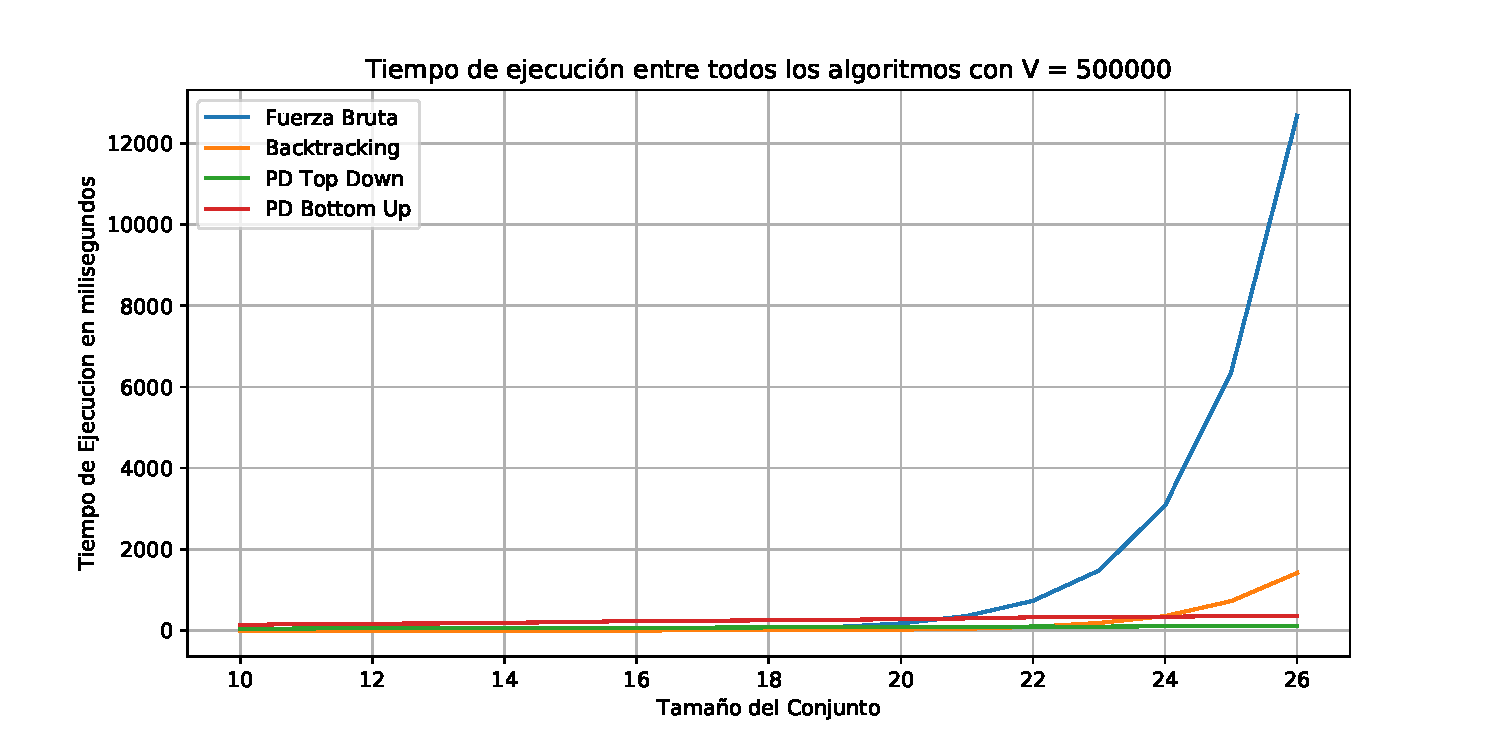
\includegraphics[width=.8\linewidth]{G3.pdf}
\end{center}

Si bien este gráfico no nos dice mucho de como son los dos algoritmos de programación dinámica, nos ayuda a ver que aún tomando datos de $V$ grandes son mejores que la Fuerza Bruta y Backtracking. El tamaño del conjunto no llega a crecer mucho ya que como la Fuerza Bruta pasa por todos los subconjuntos de partes de $S$ la cantidad de pasos que tiene que realizar crece demasiado rápido, al punto de que no alcanza la memoria del sistema para poder calcularlos, esto no pasa de la misma forma con los otros algoritmos.
\\
Ya que los algoritmos Top Down y Bottom Up resultaron mejores, nos interesaría saber cuál de ellos es mejor, para eso se hicieron dos experimentos, uno donde se altera la cantidad de elementos del conjunto y otro donde se altera el valor objetivo del problema.
\\
El primer experimento produjo el suguiente gráfico:

\begin{center}
	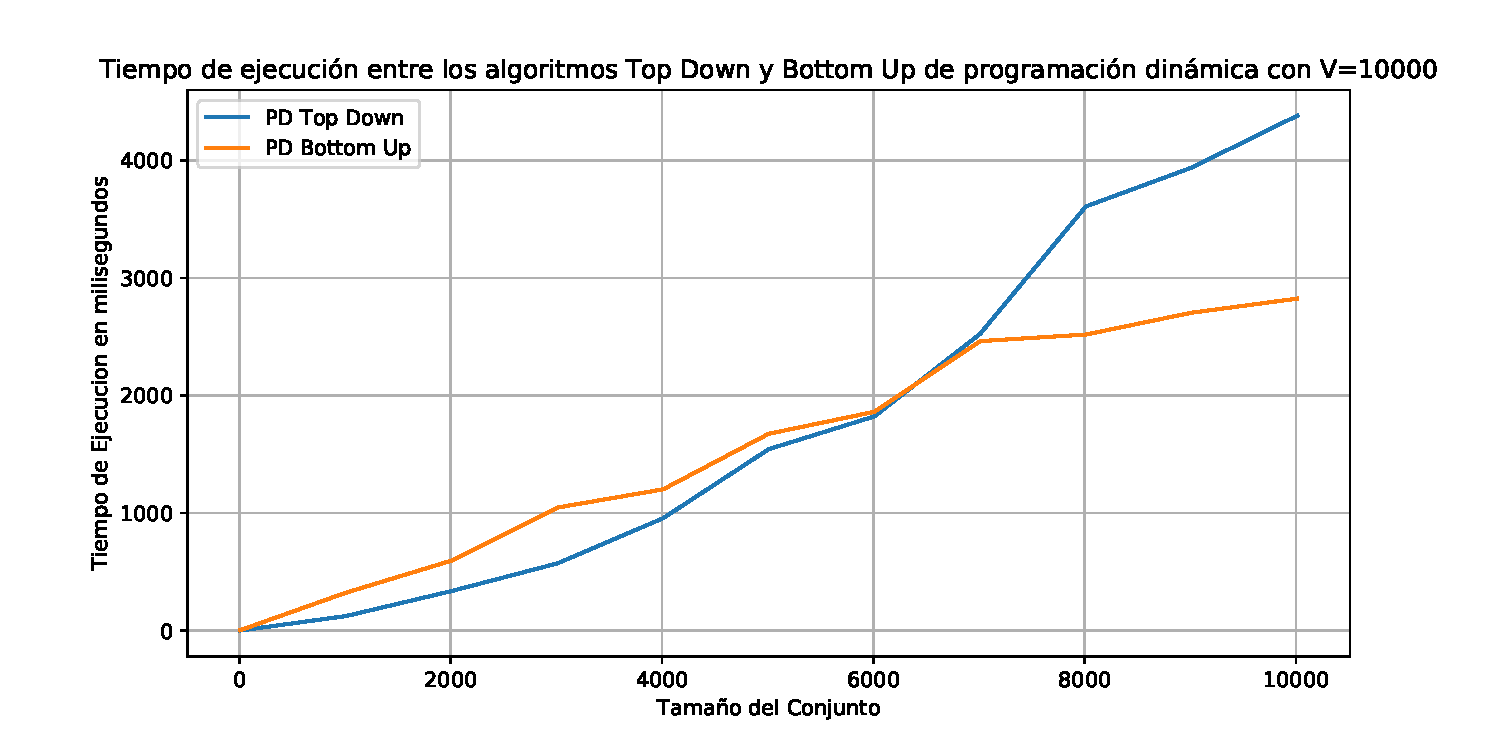
\includegraphics[width=.8\linewidth]{G2.pdf}
\end{center}

Y el segundo produjo este:

\begin{center}
	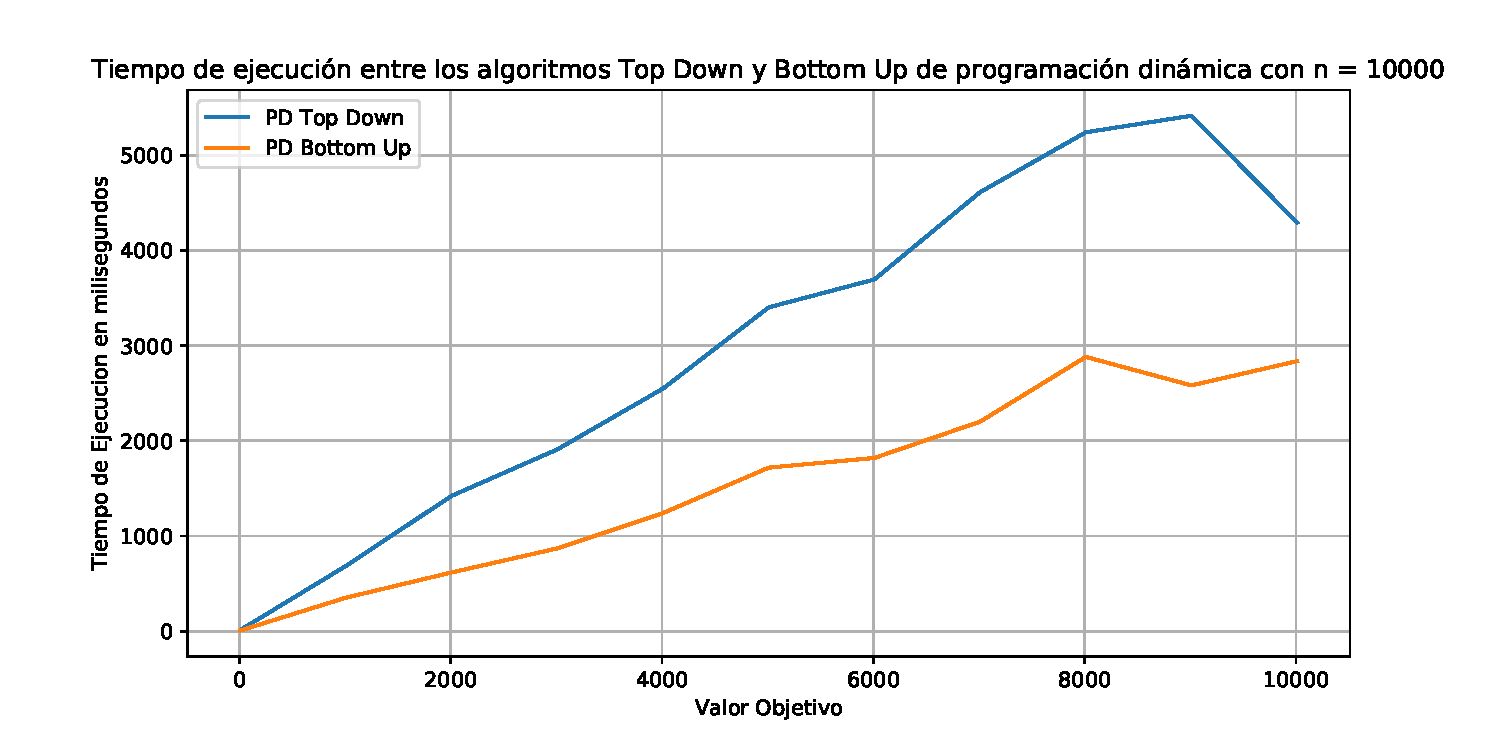
\includegraphics[width=.8\linewidth]{G4.pdf}
\end{center}

De estos gráficos podemos ver que a la larga el algoritmo Bottom Up es el que termina resolviendo el problema en menos tiempo, pero lo que es más interesante es que los dos algoritmos tienden a tardar más a media que aumenta el valór $V$ que si aumenta la cantidad de elementos en el conjunto. En el caso del algoritmo Top Down, en el primér gráfico se ve que llega a tardar como mucho unos $4.5$ segundos mientras que en el segundo se ve que se pasa de los $5$ segundos en una ocasión.
\\
Esto puede estar sucediendo porque el algoritmo Top Down depende del valor $V$ para ir llegando a los casos base, mientras que el Bottom Up llena su matriz siempre al mismo paso, aunque esto le saque ventaja cuando $V$ no es muy grande.

Luego de la experimentación podemos concluir que el algoritmo más óptimo para resolver el problema de Subset Sum en general es el Bottom Up, aunque los otros métodos podrían ser utilizados si se tiene conocimiento sobre cuales van a ser los datos de entrada, por ejemplo si se supiera que el conjunto va a tener muchos 0 el algoritmo de Backtracking podría ser utilizado y aún se obtendrian resultados en tiempos rápidos.

%\section{Conclusiones}
%Acá van las conclusiones (si las hay)

%\section{Código}

%\lstinputlisting[language=C++]{main.cpp}

\end{document}
